\section*{Zadanie 17.}
\begin{task}
Przedyskutować fizyczne implikacje prawa Ampera w różnych przypadkach.\\
\end{task}

\begin{solution}
Drugie równanie Maxwella otrzymujemy z prawa Ampere`a mówiącego o związku między przepływającym prądem a polem magnetycznym wytwarzanym przez ten prąd. Prawo to ma następującą postać:
$$\oint_{l}\vec{H}d\vec{l}=I=\iint_{s}\vec{J}\vec{n}ds$$
$$\vec{J}=\vec{J_{d}}+\vec{J_{p}}+\vec{J_{u}}$$\\
$\vec{J_{p}}=\sigma\vec{E}$; $\vec{J_{u}}=\rho\vec{V}$; $\vec{J_{p}}$ - prąd przesunięcia.\\
Do wyrażenia określającego gęstość prądu przesunięcia możemy dojść rozważając proces ładowania lub rozładowywania kondensatora płaskiego. W czasie ładowania kondensatora do jego okładek dopływa prąd $I=\cfrac{dq}{dt}$. Między okładkami nie ma ładunków, prawo ciągłości prądu nie jest spełnione, dopóki nie założymy, że między okładkami kondensatora płynie także prąd o takiej samej wartości co w przewodach podłączonych do okładek, związany ze zmianami wektora indukcji elektrycznej w czasie ładowania kondensatora.\\

\begin{center}
$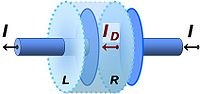
\includegraphics[scale=0.7]{17}$\\
\end{center}

$$\vec{J_{d}}=\cfrac{\partial\vec{D}}{\partial t}$$
Po sprowadzeniu gęstości prądu przesunięcia do prawa Ampere`a otrzymamy II równanie Maxwella w postaci całkowej:
$$\oint_{l}\vec{H}d\vec{l}=\iint(\vec{J}+\cfrac{\partial\vec{D}}{\partial t})\vec{n}ds, \ \vec{J}=\vec{J_{p}}+\vec{J_{u}}$$
Postać różniczkowa: $\nabla\times\vec{H}=\vec{J}$


\end{solution}

